\section{Database design}

\subsection{Rules/requirements describing the associations/relationships}

\subsubsection{Antagelser}

% beskriv antagelser omkring system HER

For at designe system mest effektivt, kiggede vi først på hvad vi faktisk kunne trække ud af serveren. Dette viste sig at være følgende attributter:

\begin{itemize}
	\item SensorId.
	\item ApartmentId.
	\item Value.
	\item Timestamp.
\end{itemize}

Af dette kom vi frem til to entities: \textit{Sensor} og \textit{Measurement}, som hver kan ses beskrevet vha. ER og UML diagram på figur~\ref{fig:erdiagram} og \ref{fig:umldiagram}.

\subsubsection{Regler}

Med dette kunne vi da opstille to regler for hvordan relationen skulle opføre sig:

\begin{itemize}
	\item Sensor can have * (Many) instances of Mesurement.
	\item Mesurement can have 1 (One) instance of Sensor.
\end{itemize}

\subsection{UML og ER diagrams}
%\subsection{Simple user stories/use case} % nødvendig?

\begin{figure}[h]
	\centering
	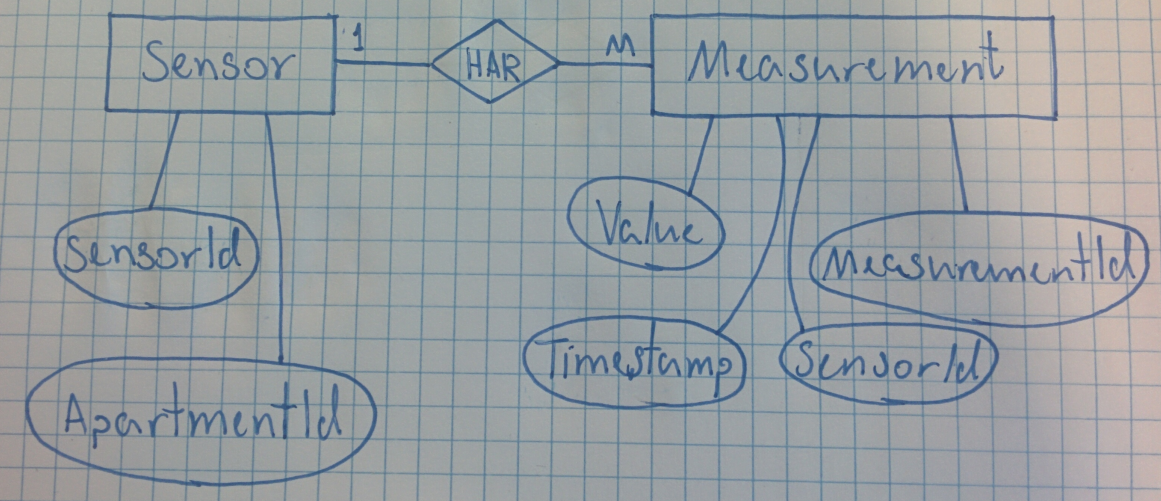
\includegraphics[width=0.8\linewidth]{figs/erdiagram}
	\caption{ER diagram for databasedesign.}
	\label{fig:erdiagram}
\end{figure}

\begin{figure}[h]
	\centering
	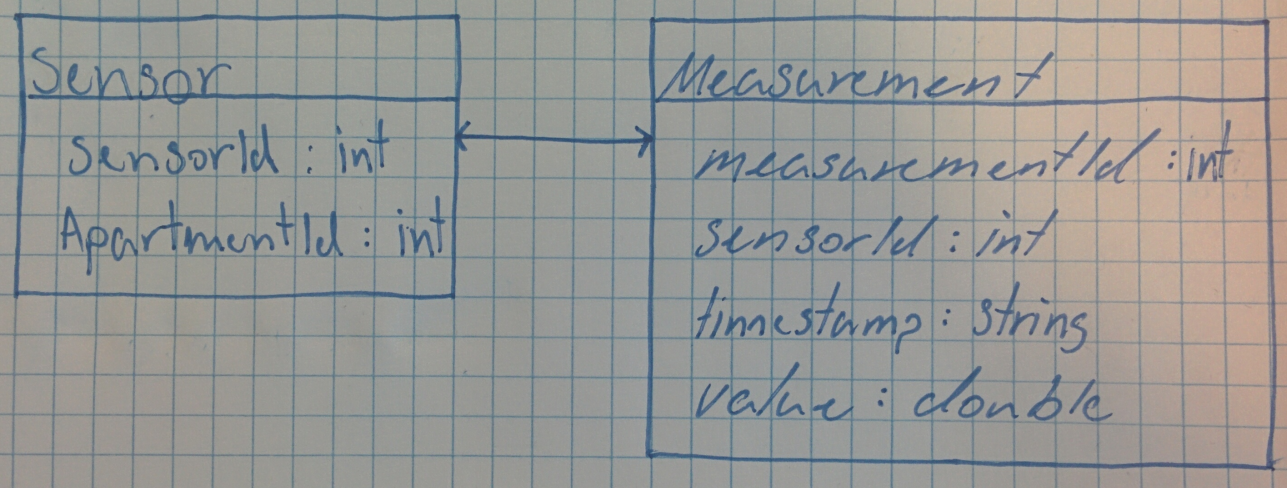
\includegraphics[width=0.8\linewidth]{figs/umldiagram}
	\caption{UML diagram for databasedesign.}
	\label{fig:umldiagram}
\end{figure}

\subsection{Stored procedures}
Der er lagt 2 stored procedures op på databasen.

\begin{itemize}
	\item GetAllData - Kalder funktionen GetData.
	\item InsertMeasurements
\end{itemize}
% some words here pree?